\section{Results: Reference Branch R1}

R1 is an exploratory reference branch rather than a uniquely derived BHSM cosmology. Its purpose is to demonstrate that the bridge can simultaneously realize late-time scalar activation, a selected physical \(n=2\) response, and near-standard high-\(n\) structure growth within the retained illustrative filter realization.

For
\[
\Omega_{m0}=0.31,\quad
\Omega_{r0}=9.0\times10^{-5},\quad
\Omega_{k0}=-0.018,\quad
\lambda=1,\quad q=3,
\]
the shooting condition \(E(1)=1\) gives
\[
\boxed{
\frac{V_0}{M_{\rm Pl}^2H_0^2}=2.39861.
}
\]

The scalar braiding and no-ghost combination evolve as shown in Table~\ref{tab:r1background}.

\begin{table}[ht]
\centering
\begin{tabular}{rrrr}
\toprule
\(z\) & \(\alpha_B\) & \(D_{\rm kin}\) & \(\Omega_T\)\\
\midrule
10  & \(2.07\times10^{-7}\) & \(1.64\times10^{-6}\) & 0.00194\\
3   & \(8.60\times10^{-5}\) & \(6.80\times10^{-4}\) & 0.03915\\
2.1 & \(3.72\times10^{-4}\) & 0.00294 & 0.08060\\
1.5 & 0.00122 & 0.00959 & 0.14321\\
1.0 & 0.00380 & 0.02988 & 0.24551\\
0.8 & 0.00622 & 0.04889 & 0.30787\\
0.5 & 0.01346 & 0.10536 & 0.43200\\
0.3 & 0.02271 & 0.17740 & 0.53538\\
0   & 0.04940 & 0.38485 & 0.70791\\
\bottomrule
\end{tabular}
\caption{Conditional reference-branch background evolution; all columns are dimensionless.}
\label{tab:r1background}
\end{table}

The scalar equation of state evolves from nearly vacuum-like behavior at high redshift to
\[
w_T(z=0)\simeq-0.906,
\]
and the background acceleration transition occurs at
\[
z_{\rm acc}\simeq0.683.
\]

Relative to a curved \(\Lambda\)CDM model with identical \(H_0,\Omega_{m0},\Omega_{r0},\Omega_{k0}\), the R1 expansion rate differs by only order one percent over the late-time interval. The maximum difference in the tabulated range is about \(1.7\%\) near \(z\sim0.5\).

\subsection{Prospective growth target}

In the minimal high-\(n\) realization, the direct topographic fifth-force term is negligible on ordinary RSD modes and the dominant growth shift is produced by the altered background history. With identical matter-era normalization,
\[
R_{f\sigma_8}(z)
=
\frac{f\sigma_{8,\rm R1}}
{f\sigma_{8,\Lambda{\rm CDM}}}
\]
is

\begin{table}[ht]
\centering
\begin{tabular}{rrr}
\toprule
\(z\) & \(R_{f\sigma_8}\) & suppression\\
\midrule
2.1 & 0.99346 & 0.65\%\\
1.5 & 0.98869 & 1.13\%\\
1.0 & 0.98164 & 1.84\%\\
0.8 & 0.97795 & 2.20\%\\
0.5 & 0.97271 & 2.73\%\\
0.3 & 0.97168 & 2.83\%\\
0.0 & 0.98482 & 1.52\%\\
\bottomrule
\end{tabular}
\caption{R1 growth forecast relative to matched curved \(\Lambda\)CDM. These values are reference-branch predictions and become formally preregistered only when reproduced by the canonical code and written to the hashed manifest.}
\label{tab:r1growth}
\end{table}

The central phenomenological result is therefore not a large generic modification of gravity. It is the combination
\[
\boxed{
\begin{gathered}
\text{enhanced horizon-scale }n=2\text{ susceptibility}\\
+\ \text{rapid high-}n\text{ recovery}\\
+\ \text{few-percent late-time growth shift}
\end{gathered}
}
\]

\begin{figure}[p]
\centering
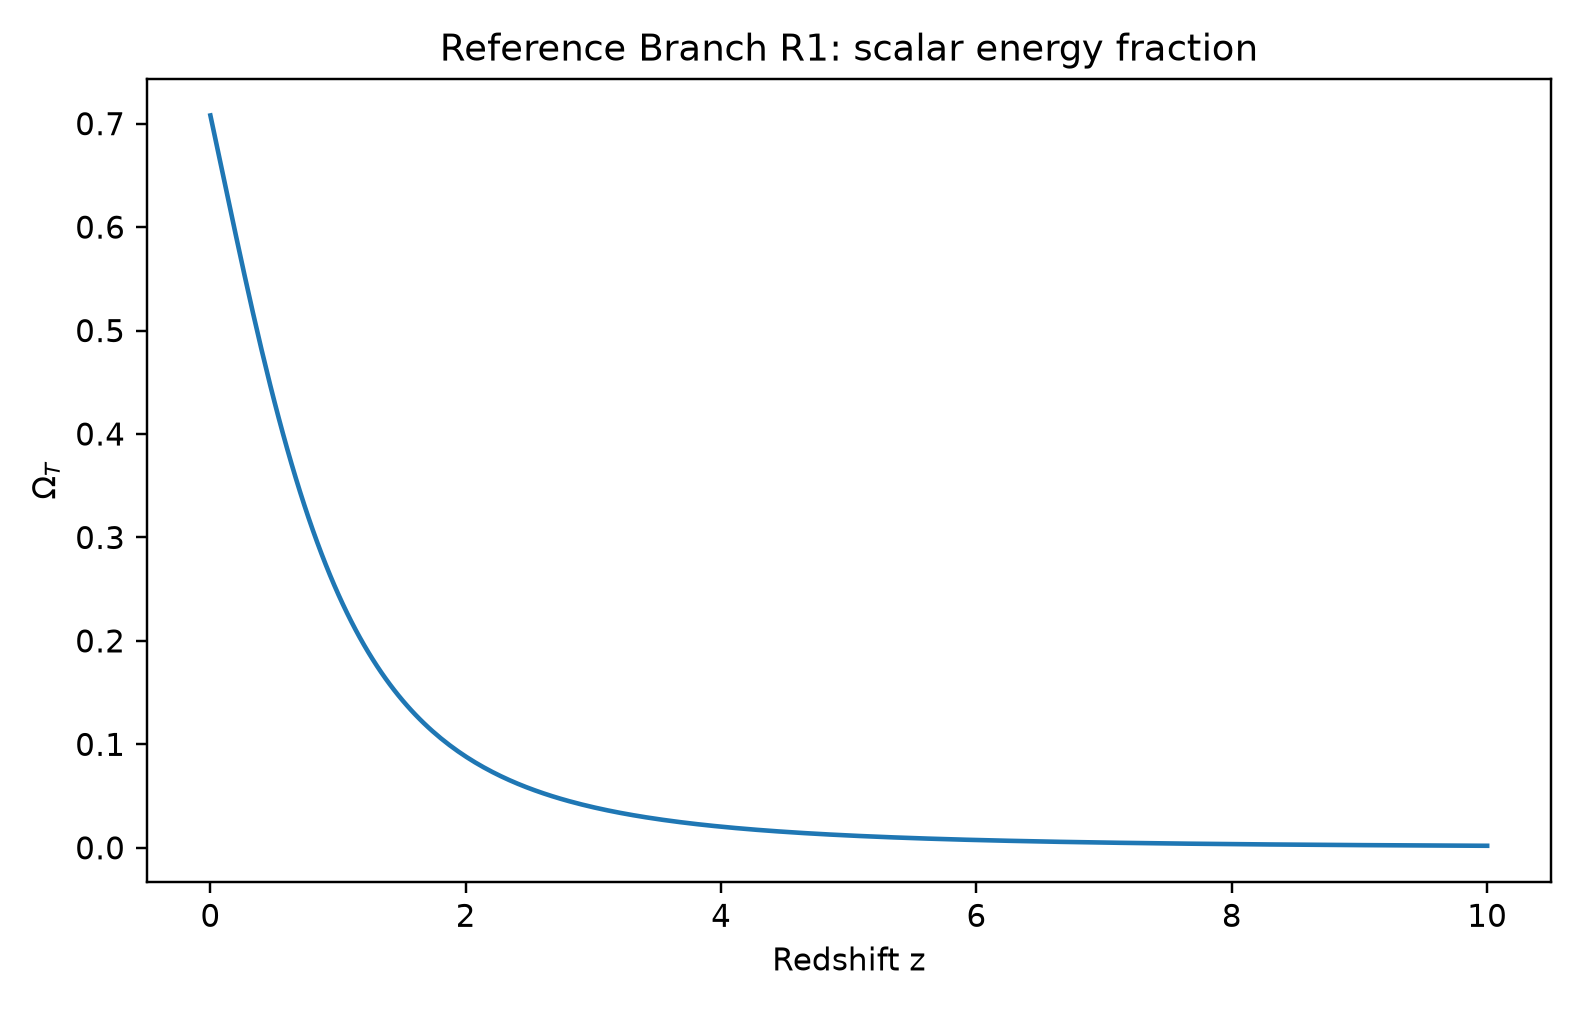
\includegraphics[width=0.82\linewidth]{figures/r1_omegaT.png}\\[0.5em]
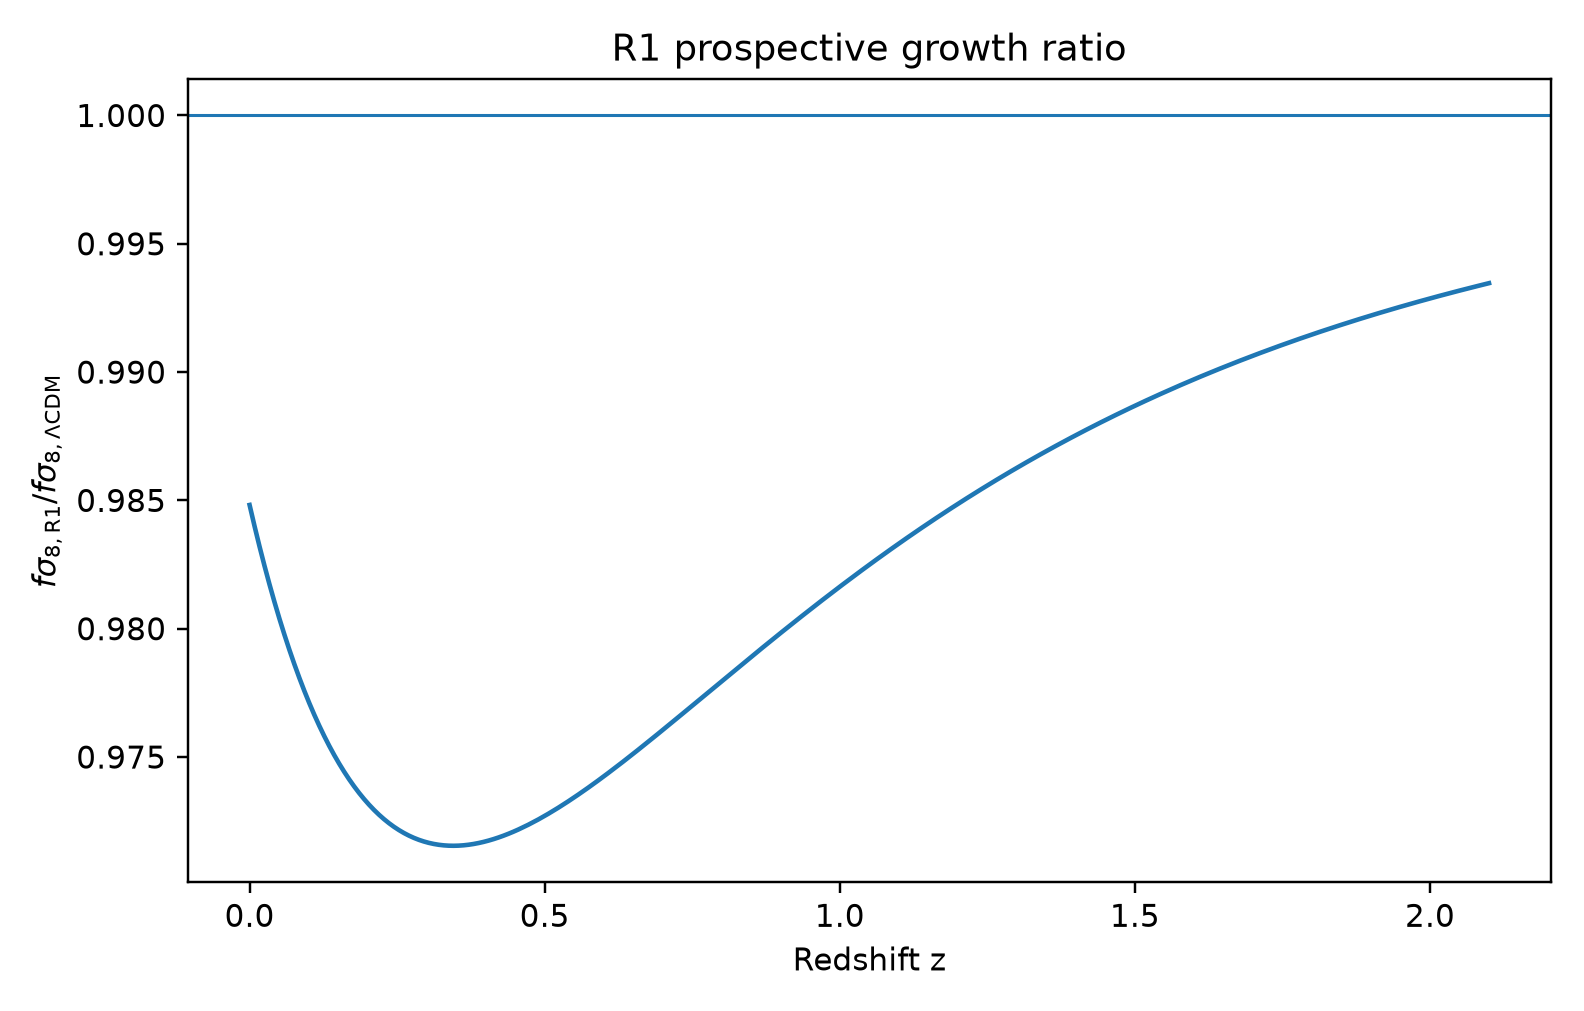
\includegraphics[width=0.82\linewidth]{figures/r1_growth_ratio.png}
\caption{Conditional frozen R1 background: scalar energy fraction (top) and growth ratio (bottom), relative to matched curved $\Lambda$CDM with identical early normalization. These are reference calculations, not fits or survey-window RSD likelihoods. Near-standard high-$n$ recovery is conditional on the illustrative retained filter.}
\label{fig:r1-background-growth}
\end{figure}

\subsection{Audited action-native quadratic stability}
Figure~\ref{fig:r1-background-growth} collects the background and reference
growth curves; Figure~\ref{fig:r1-principal-stability} shows the separate
coupled stability diagnostics.
The minimally coupled ideal dust--radiation action is reduced with the
lapse/shift Schur complement. In the retained numerical audit on
$0\le z\le2.1$, its reduced kinetic matrix is positive; the extension
through $n=1280$ has minimum eigenvalue $1.21879873\times10^{-8}$.
The principal-symbol extrapolation gives positive propagating speed
squares, with radiation approaching $1/3$ and the non-radiation branch
bounded below by approximately $0.910373$ at the sampled epochs.
The positive normalized growth tail decreases as the harmonic sequence is
extended. No ghost or high-$k$ scalar gradient instability is detected in
this audited linear/quadratic domain. These numerical checks are not a
proof of nonlinear-fluid stability, a microscopic normalization, or an
ultraviolet completion. The detailed dispersion audit is retained in
the appendix; the gravity--scalar reference kernels above remain distinct.

\begin{figure}[p]
\centering
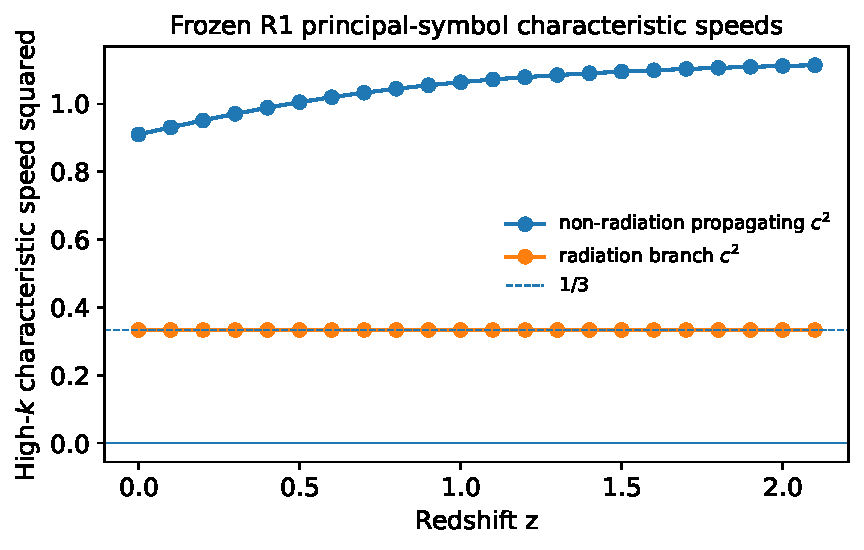
\includegraphics[width=0.82\linewidth]{figures/r1_principal_characteristic_speeds.pdf}\\[0.5em]
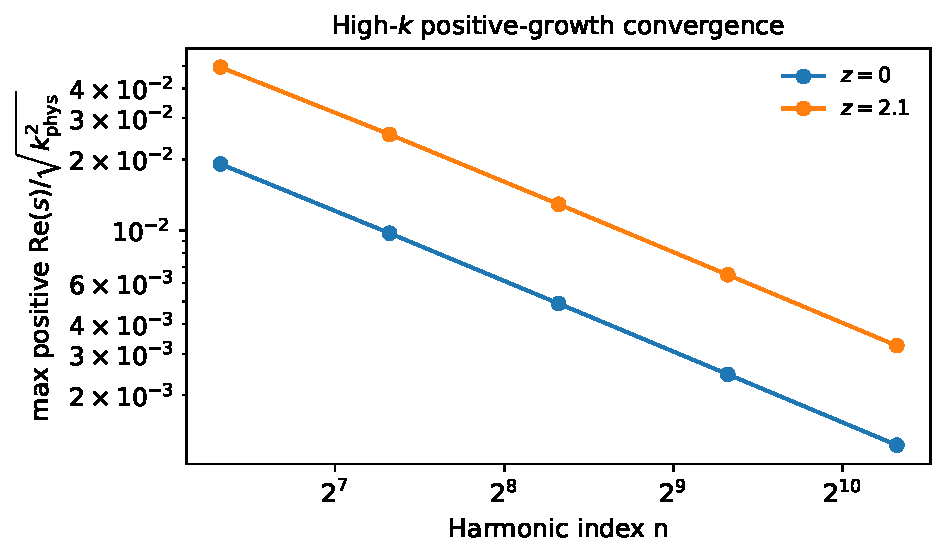
\includegraphics[width=0.82\linewidth]{figures/r1_highk_growth_convergence.pdf}
\caption{Frozen R1 coupled principal-symbol audit. Top: extrapolated characteristic speed squares at the audited redshifts, including the radiation $1/3$ reference. Bottom: the positive normalized growth tail at the two redshift endpoints decreases across the retained high-$n$ sequence. A positive finite-$n$ tail is not erased; convergence is numerical evidence within the audited quadratic domain, not an all-scale stability theorem.}
\label{fig:r1-principal-stability}
\end{figure}
